Sentiment analysis and opinion mining is the field of study that analyzes people's opinions, sentiments, evaluations, attitudes, and emotions from written language.\cite{liu2012sentiment} It's also known as emotion AI or opinion mining. The main and basic task of this field is to correctly classify the polarity of a particular text and evaluate whether is it positive, negative or in some cases neutral. It can be used in almost any situation where data need to be analyzed for its sentiment aspect - for example product reviews, online discussions or social media content.

Sentiment analysis can be divided into several standalone steps:
\begin{enumerate}
  \item \textbf{Data collection} - involves all the substeps required to gather user-generated content from any source. Surveys, blogs, various forums and social media. These all contains huge amount of real people from real world with real experiences. These data are always expressed completely different - using slang, shortcuts, internet language or generally just being used in different context.
  \item \textbf{Data preprocessing} - this step represents cleaning the data. Data preprocessing can often have a significant impact on generalization performance of a supervised ML algorithms \cite{kotsiantis2006data} and if there is much irrelevant information and data are unreliable, then knowledge discovery during the training phase is more difficult. It removes irrelevant content which could potentially lead to bad and incorrect results. This is a very delicate step because it manipulates the raw data and if not done correctly, it can easily change results.
  \item \textbf{Sentiment detection} - this step basically stands for training of the classifier. Subjective feelings and expressions are highlighted, emphasized and retained while objective information like facts are discarded and ignored. 
  \item \textbf{Sentiment classification} - subjective expressions are classified.
    \item \textbf{Output interpretation} - graphical presentation of obtained results. Time and sentiment can be analyzed to construct various charts, graphs, timelines and many other metrices.
\end{enumerate}

\subsubsection{History}


\subsubsection{Cross-correlation between releases and sentiment change}
When working with time series, we often want to determine whether one series causes changes in another. To find this relationship, measuring a cross-correlation and finding a lag is one way how to do it. Lag represents when change in one data series transfers to the other several periods later. 

To ensure a cross-correlation calculation makes sense, first I have to determine, whether are the data stationary. A stationary time series is one whose properties do not depend on the time at which the series is observed\cite{hyndman5forecast}. More precisely, if y\textsubscript{t} is a stationary time series, then for all \textit{s}, the distribution of \textit{(y\textsubscript{t},…,y\textsubscript{t+s})} does not depend on \textit{t}.

To determine whether my data are stationary, I've used the Dickey-Fuller test method of tseries package in R. Results can be seen in the table \ref{table:stationarity_table_sentiment} and \ref{table:stationarity_table_release_count} 

\begin{table}[H]
\centering
\begin{tabular}{ |p{3cm}||p{3cm}|p{3cm}|  }
 \hline
 \multicolumn{3}{|c|}{Stationarity test of web frameworks sentiment data} \\
 \hline
 Framework & Dickey-Fuller & p-value\\
 \hline
 NodeJS   & -2.6775    &0.2964\\ \hline
 AngularJS &   -3.883  & 0.0199\\ \hline
 EmberJS & -4.0783 & 0.0199\\ \hline
 VueJS    &-3.438 & 0.0646\\ \hline
 CakePHP&   -3.480  & 0.04847\\ \hline
 Laravel& -2.57  & 0.3431\\ \hline
 Symfony& -4.3979  & 0.01\\ \hline
\end{tabular}
\caption{Stationarity test of sentiment}
\label{table:stationarity_table_sentiment}
\end{table}

\begin{table}[H]
\centering
\begin{tabular}{ |p{3cm}||p{3cm}|p{3cm}|  }
 \hline
 \multicolumn{3}{|c|}{Stationarity test of web frameworks release count} \\
 \hline
 Framework & Dickey-Fuller & p-value\\
 \hline
 NodeJS   & -2.896    &0.205\\ \hline
 AngularJS &   -2.547  & 0.353\\ \hline
 EmberJS & -3.297 & 0.0802\\ \hline
 VueJS    &-2.158 & 0.511\\ \hline
 CakePHP&   -3.224  & 0.08915\\ \hline
 Laravel& -2.368  & 0.425\\ \hline
 Symfony& -2.218  & 0.488\\ \hline
\end{tabular}
\caption{Stationarity test of release counts}
\label{table:stationarity_table_release_count}
\end{table}

As we can see, p-values are always higher than 0.05 what indicates non-stationarity of the data, therefore I can't calculate the cross-correlation on them in this state. To transform non-stationary data into stationary, 2 approaches can be used. These are differencing and transforming.  I've taken data series and differenced the values in listing \ref{lst:differencing}. I've executed both, seasonal differencing and stationary differencing although seasonal probably was not needed because the data should not be dependant on the season.

\begin{lstlisting}[caption={Used differencing method in R},label={lst:differencing},language=R]
Differencing <- function(x,y)
{
 framework_x_seasdiff <- diff(x,differences=1)  # seasonal differencing
 framework_x_Stationary <- diff(framework_x_seasdiff, differences= 1)
 framework_y_seasdiff <- diff(y, differences=1)
 framework_y_Stationary <- diff(framework_y_seasdiff, differences= 1)
 return(list(framework_x_Stationary,framework_y_Stationary))
}
\end{lstlisting}
New differenced values do appear to be stationary in mean and variance, as the level and the variance of the series stays roughly constant over time. Sentiment for NodeJS before and after differencing can be seen in Figure \ref{fig:NodeJS_Sentiment_before_after}

\begin{figure}[H]%
    \centering
    \subfloat[Before differencing]{{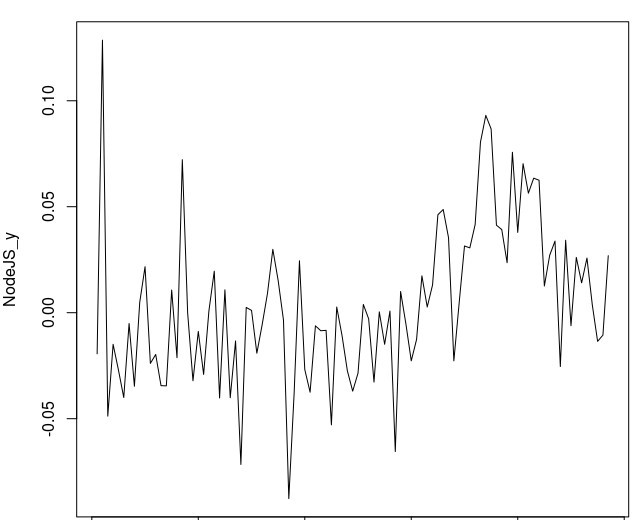
\includegraphics[width=6cm]{NodeJS_before.jpg} }}%
    \qquad
    \subfloat[After differencing]{{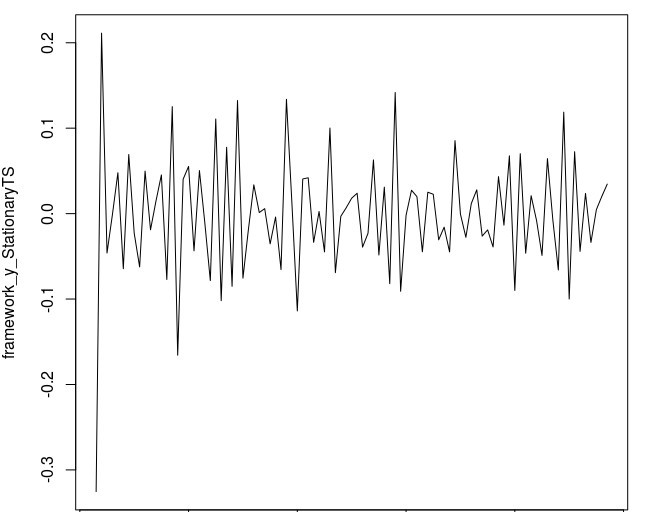
\includegraphics[width=6cm]{NodeJS_after.jpg} }}%
    \caption{NodeJS monthly sentiment values}%
    \label{fig:NodeJS_Sentiment_before_after}%
\end{figure}

Same procedure needed to be done with the "number of releases per month" data and afterwards. Then, cross-correlation could be executed. For this task I've used ccf method in R which implements Pearson's correlation calculation method. Results for all 7 OSS projects can be seen in Figure \ref{fig:highestCorrelationsPlotReleases}

\begin{figure}[H]%
    \centering
	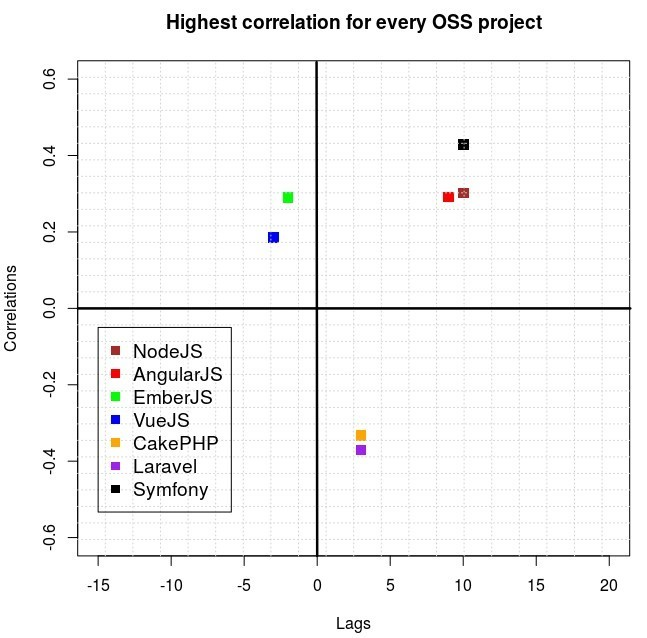
\includegraphics[width=8cm]{highestCorrelationsPlotReleases.jpg}
    \caption{Highest correlations for every OSS project}%
    \label{fig:highestCorrelationsPlotReleases}%
\end{figure}

\paragraph{Results interpretation:}

As we can there is no general pattern. Maximal project correlations happen to occupy 3 of 4 possible quadrants. Each quadrant represents a different relationship between number of releases and sentiment change.

\begin{itemize}
  \item \textbf{I. Quadrant}(Positive correlation + positive lag) - Increase of release count increases a sentiment
  \item \textbf{II. Quadrant}(Positive correlation + negative lag) - Increase of sentiment increases a release count
  \item \textbf{III. Quadrant}(Negative correlation + positive lag) - Increase of release count decreases a sentiment
  \item \textbf{IV. Quadrant}(Negative correlation + Negative lag) - Increase of sentiment decreases a release count
\end{itemize}

Also, in Figure \ref{fig:highestCorrelationsPlotReleases_nonStat} are the results without making the data series stationary. It's obvious that making the data stationary has a big impact on the results.

\begin{figure}[H]%
    \centering
	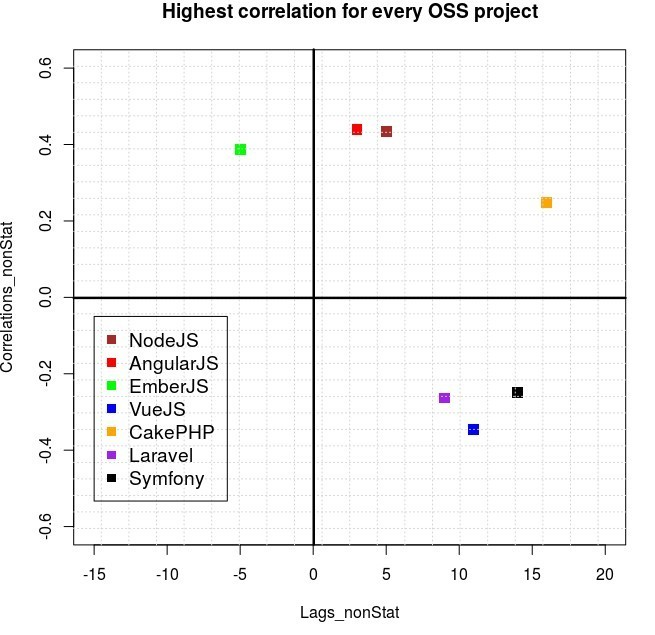
\includegraphics[width=8cm]{highestCorrelationsPlotReleases_nonStat.jpg}
    \caption{Highest correlations for every OSS project (non-stationary)}%
    \label{fig:highestCorrelationsPlotReleases_nonStat}%
\end{figure}

\subsubsection{Commits count within releases}
Initially, I thought that to modify project to take into account a size of the release (amount of commits) will be pretty straightforward task. It actually was straightforward, but as always I've encountered several unexpected problems on the way. \\
I intended to extend my previously used method from Section \ref{ssec:gitReleaseDatesMining} which uses Git API tags endpoint to get the release dates. Unfortunately I wasn't able to find number of commits in the returned objects. JSON object returned from API has following structure:
\begin{lstlisting}
  {
    "url": X,
    "assets_url": X,
    "upload_url": X,
    "html_url": X,
    "id": X,
    "tag_name": X,
    "target_commitish":X,
    "name": X,
    "draft": X,
    "author":{},
    "prerelease": X,
    "created_at": X,
    "published_at": X,
    "assets":[],
    "tarball_url": X,
    "zipball_url":X, 
    }
\end{lstlisting}
I have done some extra searching but did not want to spend extra time so I decided to go the way I knew will work. Instead of using API to get the commit counts, I crawled GitHub UI page of each release and extracted information directly from page source code. Each release details page provides information how many commits behind the current HEAD the commit is. The difference in this number between two following releases represents count of new commits for a release. Results of simple tabular substraction with spreadsheet formula needed to be manually corrected because projects often release several branches parallel and therefore substraction from the previous release was not always the correct one.\\
\\
Eventually, I got correct number of commits for every release and could execute the same cross-correlation analysis described in the previous chapter, but this time instead of releases count, I have explored relationship between sentiment and commits count. One possible flaw in the commit count data are the pre-releases. I treated them as normal releases because they do offer new features but those very same commits are then counted in the official releases later on.\\
\\
After getting the data ready I performed a stationarity test for commit counts. Sentiment values are the same as before with count of releases. Table \ref{table:stationarity_table_commits} shows the results.

\begin{table}[H]
\centering
\begin{tabular}{ |p{3cm}||p{3cm}|p{3cm}|  }
 \hline
 \multicolumn{3}{|c|}{Stationarity test of web frameworks commit counts} \\
 \hline
 Framework & Dickey-Fuller & p-value\\
 \hline
 NodeJS   & -7.0239    &0.01\\ \hline
 AngularJS &   -2.547  & 0.3531\\ \hline
 EmberJS & -3.2764 & 0.0831\\ \hline
 VueJS    &-2.9748 & 0.1886\\ \hline
 CakePHP&   -3.655  & 0.03283\\ \hline
 Laravel& -2.919  & 0.2084\\ \hline
 Symfony& -4.8461  & 0.01\\ \hline
\end{tabular}
\caption{Stationarity test of commit counts}
\label{table:stationarity_table_commits}
\end{table}

I see that there are again several data series (AngularJS, EmberJS, VueJS, Laravel + NodeJS because of unstationarity of sentiment data) which are not stationary so exactly as before with release counts, I had to transform the data. After that, Pearson's cross correlation was calculated. Results for all 7 OSS projects can be seen in Figure \ref{fig:highestCorrelationsPlot}

\begin{figure}[H]%
    \centering
	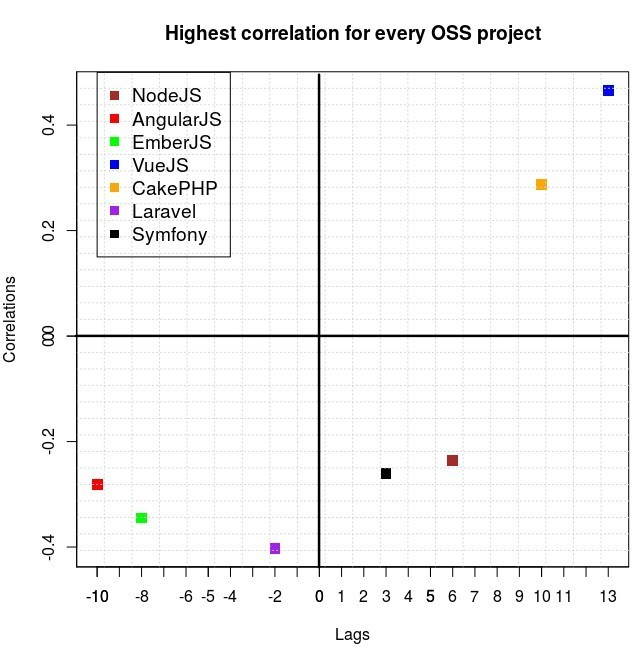
\includegraphics[width=8cm]{highestCorrelationsPlot.jpg}
    \caption{Highest correlations for every OSS project}%
    \label{fig:highestCorrelationsPlot}%
\end{figure}

If I would skip the step of making the data stationary, results would again look completely different \ref{fig:highestCorrelationsPlot_nonStat}.

\begin{figure}[H]%
    \centering
	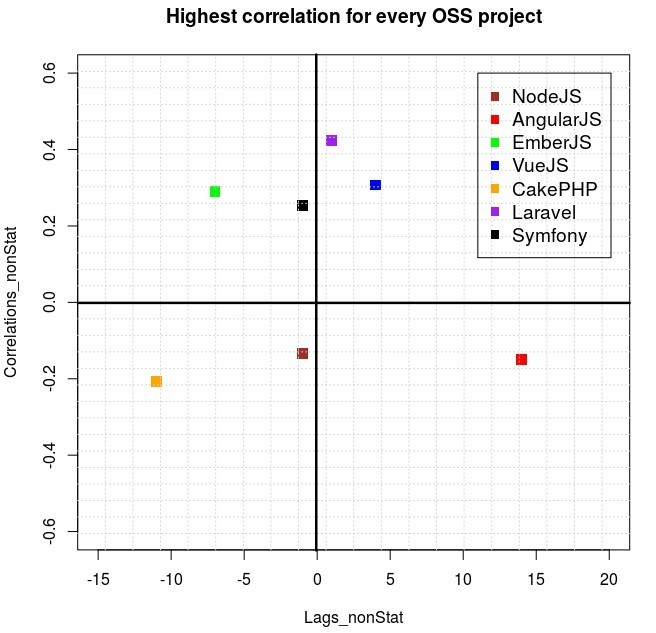
\includegraphics[width=8cm]{highestCorrelationsPlot_nonStat.jpg}
    \caption{Highest correlations for every OSS project (non-stationary)}%
    \label{fig:highestCorrelationsPlot_nonStat}%
\end{figure}
